% A simple neuralnet with one hidden layer.

\def\layersep{2.0cm}

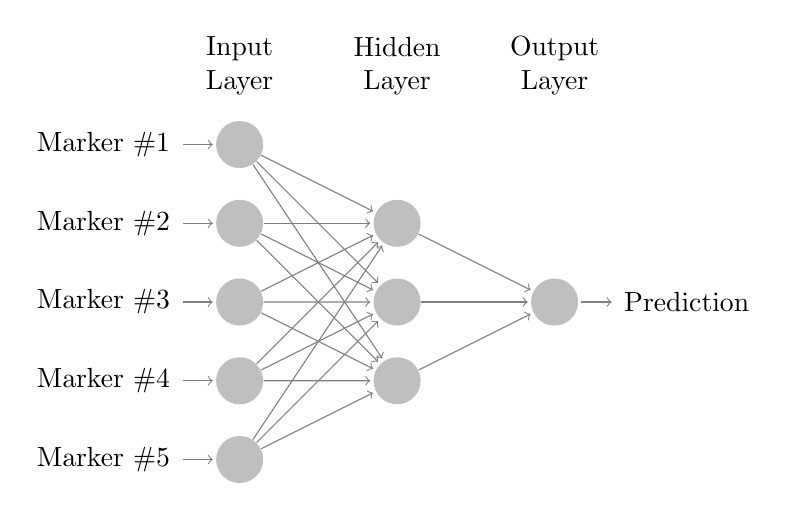
\begin{tikzpicture}[shorten >=1pt, ->, draw=black!50, node distance=\layersep]
    \tikzstyle{every pin edge}=[<-, shorten <=1pt]

    \tikzstyle{neuron}=[circle, fill=black!25,minimum size=17pt, inner sep=0pt]
    \tikzstyle{input neuron}=[neuron];
    \tikzstyle{output neuron}=[neuron];
    \tikzstyle{hidden neuron}=[neuron];

    \tikzstyle{annot}=[text width=4em, text centered]

    \foreach \name / \y in {1,...,5}
        \node[input neuron, pin=left:Marker \#\y] (I-\name) at (0,-\y) {};

    \foreach \name / \y in {1,...,3}
        \path[yshift=-1cm]
            node[hidden neuron] (H-\name) at (\layersep,-\y cm) {};

    \node[output neuron, pin={[pin edge={->}]right:Prediction}, right of=H-2] (0) {};

    \foreach \source in {1,...,5}
        \foreach \dest in {1,...,3}
            \path (I-\source) edge (H-\dest);

    \foreach \source in {1,...,3}
        \path (H-\source) edge (0);

    \node[annot, above of=I-1, node distance=1cm] (il) {Input Layer};
    \node[annot, right of=il] (hl) {Hidden Layer};
    \node[annot, right of=hl] {Output Layer};

\label{fig:simplenet}
\end{tikzpicture}

